\documentclass[aspectratio=169]{beamer}
\usepackage{tikz}
\usepackage{graphicx}
\usepackage{xypic}

\usecolortheme{whale}
\usetikzlibrary{er,positioning}  
\usetikzlibrary{decorations.pathreplacing}
\usetikzlibrary{arrows, decorations.markings}
\usetikzlibrary{shapes.geometric}
\usetikzlibrary{mindmap}

\setbeamertemplate{navigation symbols}{}

% \setbeameroption{show notes on second screen=right}

\definecolor{violet}{rgb}{0.53, 0.0, 0.69}

\definecolor{blue1}{RGB}{126,126,206}
\definecolor{blue2}{RGB}{87,87,192}
\definecolor{blue3}{RGB}{51,51,178}
\definecolor{blue4}{RGB}{27,26,107}

\tikzstyle{every link} = []
\tikzstyle{link} = [>=triangle 60, draw, every link]

\definecolor{attr}{RGB}{10,153,2}

\graphicspath{{img/}{./}} % Specifies where to look for included images (trailing slash required)

\newcommand<>{\red}[1]{\textcolor#2{red}{#1}}
\newcommand<>{\green}[1]{\textcolor#2{green}{#1}}
\newcommand<>{\gray}[1]{\textcolor#2{gray}{#1}}


\title{Bases de Datos}
\subtitle{Fundamentos de los Modelos No-relacionales. Relacional vs. No-relacional. ACID vs. BASE}
\author[Garc\'ia L., Cardentey V. M., Ledesma. A]{
    Lic. Andy Ledesma Garc\'ia\\ 
    Lic. V\'ictor M. Cardentey Fundora\\ 
    Dra. C. Lucina Garc\'ia Hern\'andez
}
\institute[MATCOM-UH]{
    Departamento de Computaci\'on\\
    Facultad de Matem\'atica y Computaci\'on\\
    Universidad de La Habana\\[3mm]
    Licenciatura en Ciencia de Datos
}
\date[]{5 de marzo de 2024}


\begin{document}
    \maketitle
    
\section{Objetivos}
\begin{frame}
    \frametitle{Objetivos de la clase de hoy}

    \begin{itemize}[<+->]
        \item Reconocer la vigencia y las limitaciones de las bases de datos relacionales. 
        \item Brindar una breve panorámica de las motivaciones y los fundamentos de las bases de datos NoSQL.
        \item Mencionar los principales retos que se presentan al migrar de un sistema de gestión de bases de datos relacionales a uno NoSQL.
    \end{itemize}
\end{frame}

\section{El modelo relacional no es suficiente}
\begin{frame}
    \frametitle{Sistemas Gestores de Bases de Datos Relacionales (RDBMS)}

    \begin{columns}[t]
        \column{0.5\textwidth}
        \begin{exampleblock}{Pros}
            \begin{itemize}[<+(1)->]
                \item Estructura bien definida 

                \item Integridad de los datos 

                \item Consultas complejas 

                \item Escalabilidad vertical

                \item ACID 

                \item Seguridad 

                \item Madurez
            \end{itemize}
        \end{exampleblock}
        \column{0.5\textwidth}
        \begin{alertblock}{Contras}
            \begin{itemize}[<+(1)->]
                \item \textcolor<-13>{red}{Costos} de licencia, hardware y administración 
                \item \textcolor<-13>{red}{Complejidad} en el dise\~no, implementación y mantenimiento
                \item \textcolor{red}{Limitada escalabilidad horizontal} para aplicaciones distribuidas que manejan grandes volúmenes de datos 
                \item \textcolor<-13>{red}{Bajo rendimiento} para aplicaciones que requieren transacciones r\'apidas o lidian con datos no estructurados
                \item \red<-13>{Poca flexibilidad} a la hora de adaptarse a cambios en la estructura
            \end{itemize}
        \end{alertblock}
    \end{columns}

    \pause
\end{frame}

\section{Teorema de CAP}

\subsection{Bases de datos distribuidas}
\begin{frame}
    \frametitle{Bases de datos distribuidas}

    \begin{columns}
        \column{.6\textwidth}
        \centering
        
\includegraphics[height=\textheight]{distributed-db.jpg}

        \column{.4\textwidth}
        \centering

        \huge
        \only<2->{?`Ventajas?\\[10mm]}

        \only<3->{?`Problemas?}
    \end{columns}

\end{frame}
\subsection{Teorema CAP}
\begin{frame}
    \frametitle{El Teorema de CAP}

    \begin{columns}
        \column{.6\textwidth}
        \centering
        \includegraphics<2-10>[height=\textheight]{distributed-db.jpg}

        \column{.4\textwidth}
        \centering

        \only<3->{
            \only<7->{{\Large Elige 2:}}
        \begin{itemize}
            \item \red<4,8,9>{Consistencia} \only<3>{(\textit{\red{C}onsistency})}
            \item \red<5,8,10>{Disponibilidad} \only<3>{(\textit{\red{A}vailability})}
            \item \red<6,9,10>{Tolerancia a particiones} \only<3>{(\textit{\red{P}artition tolerance})}
        \end{itemize}

        }
        \only<7>{
        \begin{flushright}
            \small
            \textit{por Eric Brewer, 2000;}

            \textit{demostrado por Seth Gilbert y Nancy Lynch, 2002.}
        \end{flushright}
        }
    \end{columns}

\end{frame}

\begin{frame}
    \frametitle{El Teorema de CAP}

    \centering
    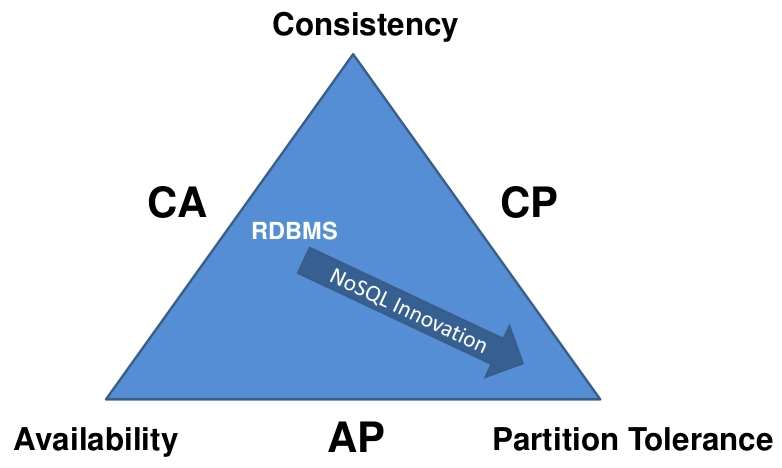
\includegraphics[scale=.7]{cap-theorem.jpg}

\end{frame}

\section{ACID vs. BASE}
\begin{frame}
    \frametitle{ACID vs. BASE}

    \begin{columns}
        \column{.5\textwidth}

        \begin{block}{ACID}
            \begin{itemize}
                \item \textit{\red{A}tomicity}
                \item \textit{\red{C}onsistency}
                \item \textit{\red{I}solation}
                \item \textit{\red{D}urability}
            \end{itemize}
        \end{block}

        \column{.5\textwidth}

        \begin{block}{BASE}
            \begin{itemize}
                \item \textit{\red{Ba}sically Available}
                \item \textit{\red{S}oft state}
                \item \textit{\red{E}ventual consistency}
            \end{itemize}
        \end{block}
    \end{columns}

\end{frame}

\begin{frame}
    \frametitle{ACID vs. BASE}

    \centering
    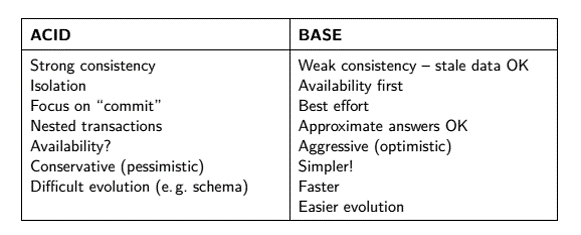
\includegraphics[width=\textwidth]{acid-vs-base.jpg}
\end{frame}

\section{Fundamentos de los modelos no-relacionales}
\begin{frame}
    \centering
    \Huge Paradigma NoSQL

\end{frame}

\begin{frame}
    \frametitle{Paradigma NoSQL}

    \centering
    \Huge NoSQL \only<1>{$=$ ?`?}\only<2>{$\neq$ No to SQL}\only<3>{$=$ Not only SQL}

\end{frame}

\begin{frame}
    \frametitle{ACID vs. BASE}

    \centering
    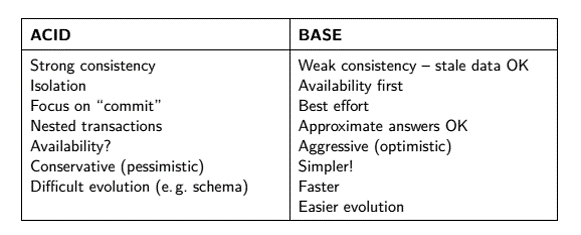
\includegraphics[width=\textwidth]{acid-vs-base.jpg}
\end{frame}

\begin{frame}
    \frametitle{SBD NoSQL}

    \begin{block}{Usos frecuentes}
        \pause
        \begin{itemize}[<+->]
            \item Escenarios con nuevos problemas en la organización
            \item Carga de los datos previa a conocer el esquema o con gran variación
            \item Contextos donde las BDRs no aseguran  el desempeño requerido para manipular los datos actuales
            \item Dinamismo en la definición de las interrelaciones
            \item Necesidad de distribución y acceso global
        \end{itemize}
    \end{block}

\end{frame}

\begin{frame}
    \frametitle{SBD NoSQL}

    \begin{columns}
        \column{0.5\textwidth}
        \begin{exampleblock}{Pros}
        \begin{itemize}
            \item Escalabilidad
            \item Flexibilidad
            \item Alto Rendimiento
            \item Agilidad
            \item Adecuado para Big Data y aplicaciones en tiempo real
        
        \end{itemize}
        \end{exampleblock}
        
        \column{0.5\textwidth}
        \begin{alertblock}{Contras}
        \begin{itemize}
            \item Problemas de consistencia
            \item Complejidad
            \item Limitaciones de consultas
            \item Soporte limitado de transacciones
            \item Desafíos en Consistencia e Integridad de Datos
        \end{itemize}
        \end{alertblock}
        
    \end{columns}
\end{frame}
\section{Retos para migrar de RDBMS a NoSQL}

    \maketitle
\end{document}